\documentclass[tikz,border=8pt]{standalone}
\usepackage{amsmath,amssymb}
\usetikzlibrary{arrows.meta,calc,decorations.markings,decorations.pathmorphing,patterns,shapes.geometric,positioning}

\begin{document}
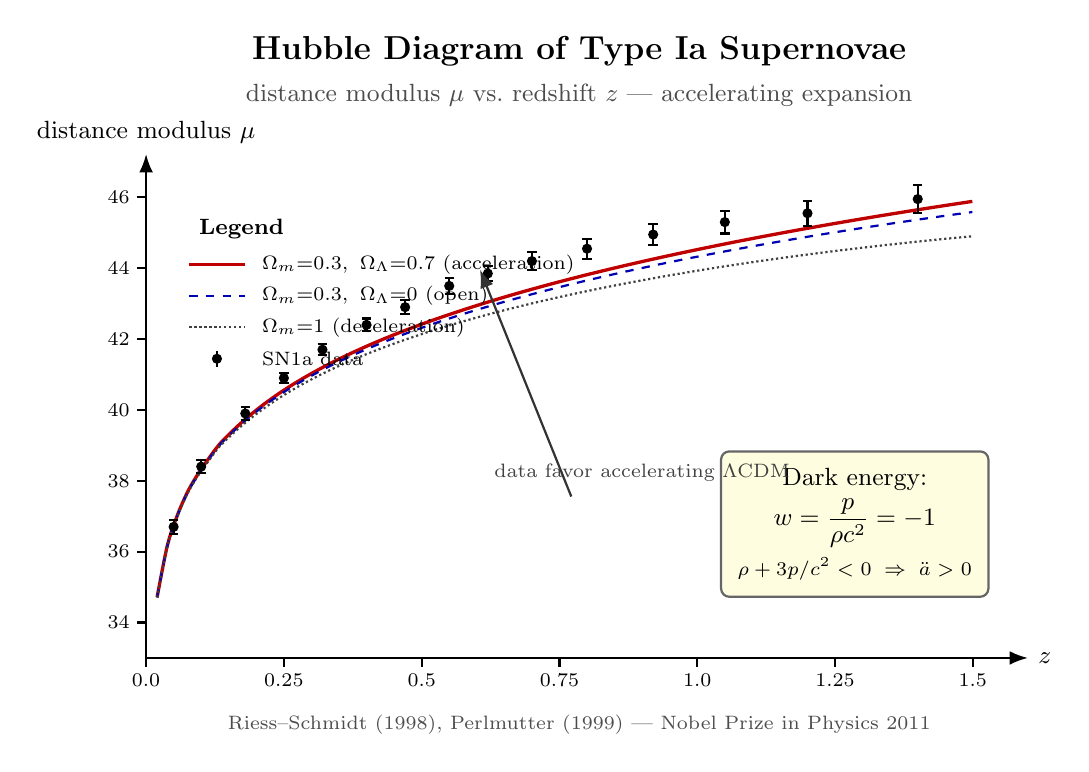
\begin{tikzpicture}[>=Latex,
  axisstyle/.style={thick, black},
  curveLCDM/.style={very thick, red!75!black},
  curveOpen/.style={thick, blue!70!black, dashed},
  curveEdS/.style={thick, gray!50!black, densely dotted},
  datapt/.style={circle, fill=black, inner sep=1.3pt},
  errbar/.style={thick, black}]

  % Title at top
  \node[font=\large\bfseries, align=center] at (5.5, 7.7)
    {Hubble Diagram of Type Ia Supernovae};
  \node[font=\small, align=center, text=black!70] at (5.5, 7.15)
    {distance modulus $\mu$ vs.\ redshift $z$ — accelerating expansion};

  % --- Plot frame, x in [0, 1.5], y in [33, 46] ---
  % Map: x = 7 * z (so z=1.5 -> x=10.5), y = (mu - 33) * 0.45 (so mu=46 -> y=5.85)
  % Origin at (0,0), x-axis goes 0..10.5, y-axis 0..5.85
  \def\xs{7.0}      % x-scale (cm per unit redshift)
  \def\yo{33}       % mu offset
  \def\ys{0.45}     % y-scale (cm per mag)

  % Axes
  \draw[axisstyle, ->] (0, 0) -- (11.2, 0) node[right, font=\small] {$z$};
  \draw[axisstyle, ->] (0, 0) -- (0, 6.4) node[above, font=\small] {distance modulus $\mu$};

  % x-ticks
  \foreach \z in {0.0, 0.25, 0.5, 0.75, 1.0, 1.25, 1.5} {
    \draw[axisstyle] (\z*\xs, 0) -- (\z*\xs, -0.12);
    \node[font=\scriptsize, below=1pt] at (\z*\xs, -0.05) {\z};
  }

  % y-ticks
  \foreach \m in {34, 36, 38, 40, 42, 44, 46} {
    \pgfmathsetmacro{\yy}{(\m - \yo) * \ys}
    \draw[axisstyle] (0, \yy) -- (-0.12, \yy);
    \node[font=\scriptsize, left=1pt] at (-0.05, \yy) {\m};
  }

  % --- Theoretical curves (approximate mu(z) for the three cosmologies) ---
  % We use simple polynomial approximations consistent with mu(z) shape in [0,1.5].

  % LambdaCDM (Omega_m=0.3, Omega_Lambda=0.7) -- highest of the three at high z
  \draw[curveLCDM]
    plot[domain=0.02:1.5, samples=80, smooth] (\x*\xs,
      {(43.16 + 5*ln(\x*(1+0.5*\x)*(1 + 0.30*\x - 0.05*\x*\x))/ln(10) - \yo)*\ys});

  % Open (Omega_m=0.3, Omega_Lambda=0): middle
  \draw[curveOpen]
    plot[domain=0.02:1.5, samples=80, smooth] (\x*\xs,
      {(43.16 + 5*ln(\x*(1+0.5*\x)*(1 + 0.20*\x - 0.06*\x*\x))/ln(10) - \yo)*\ys});

  % Einstein-de Sitter (Omega_m=1, Omega_Lambda=0): lowest
  \draw[curveEdS]
    plot[domain=0.02:1.5, samples=80, smooth] (\x*\xs,
      {(43.16 + 5*ln(\x*(1+0.5*\x)*(1 + 0.05*\x - 0.10*\x*\x))/ln(10) - \yo)*\ys});

  % --- SN1a data points (illustrative; sit on the LambdaCDM curve with scatter) ---
  % each entry: z, mu, errbar
  \foreach \z/\m/\e in {%
    0.05/36.7/0.20,
    0.10/38.4/0.18,
    0.18/39.9/0.18,
    0.25/40.9/0.15,
    0.32/41.7/0.16,
    0.40/42.4/0.18,
    0.47/42.9/0.20,
    0.55/43.5/0.22,
    0.62/43.85/0.22,
    0.70/44.20/0.25,
    0.80/44.55/0.28,
    0.92/44.95/0.30,
    1.05/45.30/0.32,
    1.20/45.55/0.35,
    1.40/45.95/0.40} {
    \pgfmathsetmacro{\xx}{\z*\xs}
    \pgfmathsetmacro{\yy}{(\m - \yo)*\ys}
    \pgfmathsetmacro{\eu}{(\m + \e - \yo)*\ys}
    \pgfmathsetmacro{\ed}{(\m - \e - \yo)*\ys}
    \draw[errbar] (\xx, \ed) -- (\xx, \eu);
    \draw[errbar] (\xx-0.06, \eu) -- (\xx+0.06, \eu);
    \draw[errbar] (\xx-0.06, \ed) -- (\xx+0.06, \ed);
    \node[datapt] at (\xx, \yy) {};
  }

  % --- Legend (upper-left inside plot) ---
  \begin{scope}[shift={(0.55, 5.45)}]
    \node[anchor=west, font=\footnotesize] at (0, 0)
      {\textbf{Legend}};
    \draw[curveLCDM] (0, -0.45) -- (0.7, -0.45);
    \node[anchor=west, font=\scriptsize] at (0.8, -0.45)
      {$\Omega_m{=}0.3,\ \Omega_\Lambda{=}0.7$ (acceleration)};
    \draw[curveOpen] (0, -0.85) -- (0.7, -0.85);
    \node[anchor=west, font=\scriptsize] at (0.8, -0.85)
      {$\Omega_m{=}0.3,\ \Omega_\Lambda{=}0$ (open)};
    \draw[curveEdS] (0, -1.25) -- (0.7, -1.25);
    \node[anchor=west, font=\scriptsize] at (0.8, -1.25)
      {$\Omega_m{=}1$ (deceleration)};
    \node[datapt] at (0.35, -1.65) {};
    \draw[errbar] (0.35, -1.55) -- (0.35, -1.75);
    \node[anchor=west, font=\scriptsize] at (0.8, -1.65)
      {SN1a data};
  \end{scope}

  % --- Equation-of-state callout (right side) ---
  \node[draw=black!60, thick, rounded corners=3pt, fill=yellow!12,
        inner sep=6pt, font=\small, align=center] at (9.0, 1.7) {%
    Dark energy: \\[2pt]
    $w = \dfrac{p}{\rho c^{2}} = -1$ \\[3pt]
    \scriptsize $\rho + 3p/c^{2} < 0 \;\Rightarrow\; \ddot a > 0$%
  };

  % --- Annotation arrow pointing at LCDM-curve at z~0.6 ---
  \pgfmathsetmacro{\xa}{0.62*\xs}
  \pgfmathsetmacro{\ya}{(43.85 - \yo)*\ys}
  \draw[->, thick, gray!40!black] (5.4, 2.05) -- (\xa-0.1, \ya+0.05);
  \node[anchor=west, font=\scriptsize, text=black!75] at (4.3, 2.35)
    {data favor accelerating $\Lambda$CDM};

  % --- Discoverers footer ---
  \node[font=\scriptsize, align=center, text=black!70] at (5.5, -0.85)
    {Riess--Schmidt (1998), Perlmutter (1999) — Nobel Prize in Physics 2011};

\end{tikzpicture}
\end{document}
